\chapter{Future Work}
\label{chap:FutureWork}

In this chapter, we take up different possibilities and approaches to how the presented work around Shila can be improved and extended. The discussion refers to the results that were obtained in the course of this work and intends to provide the best possible basis for the further development of Shila.

\subsection*{Further Testing}

After completing the implementation, we checked and ensured the basic functionality of Shila with tests both in local and SCIONLab infrastructure. However, during the execution of the Shila-Measurement, as presented in the previous chapter, individual experiments occasionally failed. Of course, such experiments were repeated and not included in the measurements. The exact reasons for the failure have not been investigated in the course of this work, but the failed experiments have all been documented. An important part of the revision and further development of Shila is to use this documentation to identify and fix possible weaknesses and bugs. Hereby, the infrastructure developed for the execution of the measurements can be optimally used to perform further extensive test runs.

\subsection*{Further Measurements}

One goal of the measurements was to determine the influence of the path selection algorithm on the performance of Shila. Within the SCIONLab network, no influence could be detected. This is also due to the fact that the values of the metrics for different path options did not differ, e.g. all paths had the same value for MTU. For more comprehensive statements about the influence of the path selection further measurements are recommended. It is thereby important to consider whether the metrics used are the right ones for performance optimization or whether alternatives might be more suitable. For example, not only criteria relating to the static state of the network are conceivable. An interesting direction for further measurements could include investigations about the existence and influence of more dynamic criteria, offering more insight about the current health of the network than its static topology. Of course, the topology of the network also plays a decisive role in the investigation. If a topology offers a greater variety of different paths, it is easier to determine a possible influence of the path selection.

\subsection*{More flexible Routing-Information}

In the current version of Shila, there is only one way to pass the Routing-Information, i.e. the mapping from TCP address to SCION address. The information has to be passed along with the startup of the shim layer. This assumes that the mapping is already known and brings along a restriction in flexibility.  

One possible solution was investigated in the conceptual phase of the thesis: The record route option of the IP protocol allows to log the route of a datagram through the Internet. When enabled, each IP datagram has space in its header to store up to eight IP addresses that it encounters on its way from sender to receiver. A predefined data structure has to be specified during the creation of the socket to activate this non-compulsory socket option. This structure describes the 32 bytes of memory required for storing the addresses and can instead of the usual zero also be initialized with the SCION target address. Each packet sent from the socket created with this option contains the SCION destination address in its IP header. The SCION target address for a new Main-Flow can then be extracted by Shila from the first intercepted datagram. With a wrapper around the standard TCP API, the process of additional address specification can be made pleasant for the user. Of the 32 bytes of the record route option, 28 bytes can be used effectively. The first four bytes are overwritten when traversing the virtual interface on the way to Shila. A SCION address requires a maximum of 20 bytes. With this approach its therefore possible to pass further control information, up to eight bytes, from the application to Shila. At first glance, this approach has the disadvantage of increasing the overhead. But there is nothing to be said against reassembling the IP packet in Shila without the additional option. The stated approach is not yet part of the implementation since it is not strictly needed for the basic functionality. But once part of Shila, it increases the flexibility and possibilities of the shim layer.

\subsection*{Reducing Overhead}

As stated in the previous chapter, the data exchange with MPTCP over SCION comes with comparatively high overhead. This is also due to the multiple nesting of the payload within a SCION packet: It contains a Shila-Message\footnote{A Shila-Message is the message sent between two Shila instances via the Backbone-Connection.}, which itself holds a TCP segment in an IP datagram. The actual data sits inside the TCP packet. In this nesting, information which does not necessarily has to be transmitted is sent along. It is not mandatory to include the source and destination address in the IP header, these are defined by the TCP-Flow of the Backbone-Connection. The same applies to the protocol identification number or the checksum, which can be recalculated. An approach to reduce overhead would therefore be going without the IP header but just the TCP segment as payload and a custom header. Such a header holds only the information required to reassemble the IP packet at the receiving endpoint. An IP header without additional options has a size of 20 bytes. The identification value (2 bytes) and the flags together with the fragment offset (2 bytes) must be included in the custom header for every IP datagram processed by Shila. The remaining information necessary for the re-composition of the IP packet at the destination endpoint can either be calculated, e.g. the checksum, or is given through to the Backbone-Connection, e.g. source and destination address. With this approach, the contribution of the IP header to overhead can be reduced by 80\%. Redundant information is also sent in the TCP segment, the source and destination ports are also given by the Backbone-Connection. But the savings potential for combining the TCP header is lower, as the majority of the fields contain dynamic information. If the proposal under discussion is implemented, the additional effort for parsing and recompiling the IP datagrams should not be disregarded.
	
\subsection*{No Namespaces}

In the current implementation of Shila, the ingress interface is always assigned to the same IP address. Any TCP client starting a new data exchange via MPTCP over SCION specifies this address as the destination for the connection. Since the ingress and egress interfaces are per default located in a different namespace, this is fine. The client's traffic is routed to one of the dedicated egress interfaces and intercepted by Shila from where it is processed as intended. But if the interfaces are not separated, the traffic is routed only locally. Since the ingress interface matches the destination address (specified by the TCP client on the same host), the traffic is never about to be sent out via an interface and therefore cannot be intercepted by Shila. One possible approach to solve this problem is to adjust the local routing. We have decided against this intervention into the basic setup of the host. Another approach would be to extract the address (for the ingress interface) from the host SCION address. However, for hosts from different ASes, this is not necessarily different and therefore the problem is not solved.  With the current implementation, Shila only works without namespaces if a unique address for the ingress interface is configured on each host by hand. On a larger scale, this approach is not suitable. It is therefore required to invest further in a version of Shila that works without namespaces and does not require a manual assignment of IP addresses.

\subsection*{Side-by-side}

To conclude this chapter, we present an approach how the traditional Internet and SCION can be used side-by-side using Shila and MPTCP. In contrast to the use case presented in this thesis, the side-by-side approach realizes the main-flow of an MPTCP connection via the conventional Internet. The SCION network is only used for possible sub flows. With such an approach the establishment of SCION could be further advanced. The new technology will become better known and will ideally contribute to improved user experience without interfering with a users (and applications) known working environment. Below we outline, supported by the illustration in Figure \ref{fig:SideBySide}, how such a side-by-side solution would work.

\begin{figure}[H]
	\begin{center}
		\def\svgwidth{1\textwidth}
		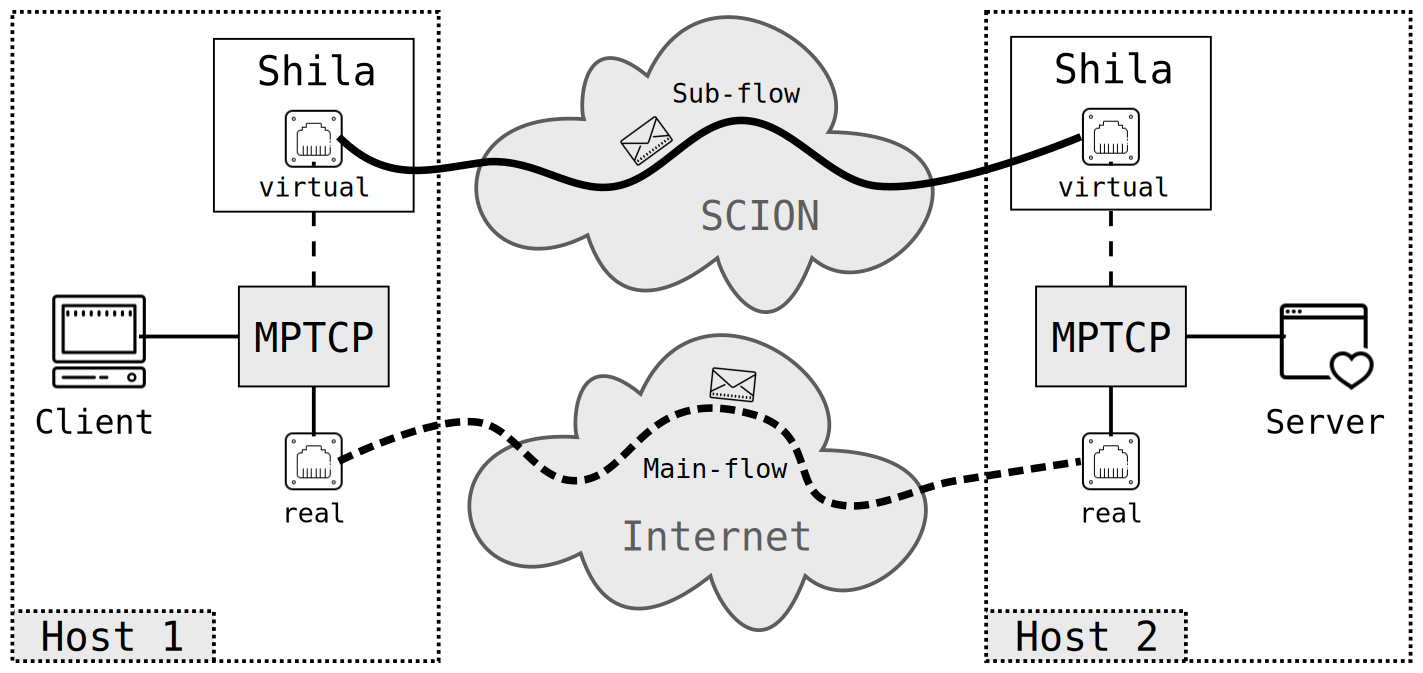
\includegraphics[scale=0.24]{../illustrations/futureWork/SideBySide.pdf}   
		\caption[]{Illustration of the side-by-side approach. The main-flow of an MPTCP connection goes through the Internet, whereas the sub-flow (possibly multiple) goes through the SCION network. The user will not experience any change in his usual working environment, but can still benefit from any possible advantages of SCION.}
		\label{fig:SideBySide}
	\end{center}
\end{figure}

We assume the following starting position: Two hosts, A and B, both part of the conventional Internet but also part of the SCION network. For access to the conventional Internet, the hosts have a corresponding real network interface.  In addition, both hosts run Shila without using namespaces for their virtual network interfaces. On Host A, a client application now initiates a connection with the server application on Host B. MPTCP establishes a main-flow over the two real interfaces. To ensure that the initial connection is established over the real interface, the client specifies the appropriate interface when connecting.\footnote{For example by specifying the interface in the \textit{connect(..)} call.} As soon as the main-flow is established, MPTCP starts trying to connect sub-flows between all the different pairs of interfaces. The Shila instance on Host A intercepts the sub-flow connection tries\footnote{MPTCP also tries to establish a sub-flow between the two virtual - real interface pairs. These attempts are ignored by the respective Shila instances after any useful information has been extracted.} coming from its virtual interface. For the one directed towards the virtual interface of Host B, it can now create a backbone connection with the Shila instance listening there. The MPTCP connection now consists of a  main-flow through the conventional Internet supplemented by a sub-flow through the SCION network. The application can only benefit from this; the mechanisms of MPTCP ensure that the availability of multiple paths is optimally used.  